% Genetics and enzyme kinetics problem set (English, university biology), with a tikz pedigree and a pgfplots curve.
% Headings: "Task N -- Title (P points)" in bold; parts (a), (b), ... and (i), (ii), ... (nested in Task 3).
\documentclass[11pt,a4paper]{article}
\usepackage[T1]{fontenc}
\usepackage{lmodern}
\usepackage[margin=2.3cm,top=2.0cm,bottom=2.2cm]{geometry}
\usepackage{amsmath,amssymb}
\usepackage{siunitx}
\usepackage{caption}
\usepackage{tikz}
\usetikzlibrary{arrows.meta}
\usepackage{pgfplots}
\pgfplotsset{compat=1.18}
\usepackage{enumitem}

\setlength{\parindent}{0pt}
\setlist[enumerate,1]{label=(\alph*), leftmargin=2.2em, itemsep=0.35em, topsep=0.3em}
\setlist[enumerate,2]{label=(\roman*), leftmargin=2em, itemsep=0.15em, topsep=0.15em}
\newcommand{\task}[3]{\bigskip\par\noindent\textbf{Task #1 -- #2 (#3 points)}\par\nopagebreak\smallskip}

\begin{document}

% ---- header ---------------------------------------------------------------------------
{\small BIOL 2100 \textperiodcentered{} Genetics and Biochemistry \hfill Faculty of Life Sciences}\\[-0.4em]
\rule{\linewidth}{0.6pt}\\[0.5em]
{\Large\bfseries Problem Set 3: Inheritance, Populations and Enzymes}\\[0.4em]
Hand in on Thursday, 19 November 2026, before the seminar \hfill Total: 26 points

% ---- Task 1 ---------------------------------------------------------------------------
\task{1}{Punnett squares}{6}
In pea plants, tall stems ($T$) are dominant over dwarf stems ($t$). Seed shape and seed colour are
inherited independently: round ($R$) is dominant over wrinkled ($r$), and yellow ($Y$) is dominant over
green ($y$).
\begin{enumerate}
  \item Two heterozygous tall plants are crossed ($Tt \times Tt$). Complete the Punnett square and give the
        genotype ratio and the phenotype ratio of the offspring.
\end{enumerate}
\begin{center}
\renewcommand{\arraystretch}{1.0}
\begin{tabular}{c|c|c|}
  \multicolumn{1}{c}{} & \multicolumn{1}{c}{$T$} & \multicolumn{1}{c}{$t$} \\ \cline{2-3}
  $T$ & \rule{0pt}{2.4em}\hspace{2.6em} & \hspace{2.6em} \\ \cline{2-3}
  $t$ & \rule{0pt}{2.4em} & \\ \cline{2-3}
\end{tabular}
\end{center}
\begin{enumerate}[resume]
  \item A tall plant is crossed with a dwarf plant. Half of the offspring are dwarf. What is the genotype of
        the tall parent?
  \item Two plants with the genotype $RrYy$ are crossed. What fraction of the offspring is wrinkled and green?
        What fraction is round and yellow?
  \item What fraction of the offspring of the cross in (c) is heterozygous for both genes?
\end{enumerate}

% ---- Task 2 ---------------------------------------------------------------------------
\task{2}{Hardy--Weinberg equilibrium}{6}
In a population of 1000 beetles, 160 show a recessive trait (genotype $aa$). Assume the population is in
Hardy--Weinberg equilibrium for this locus with two alleles, $A$ (dominant) and $a$ (recessive).
\begin{enumerate}
  \item Calculate the allele frequency $q$ of $a$.
  \item Calculate the allele frequency $p$ of $A$ and the expected frequencies of the genotypes $AA$, $Aa$
        and $aa$.
  \item How many of the 1000 beetles are expected to be heterozygous carriers?
  \item Name two conditions that must hold for a population to stay in Hardy--Weinberg equilibrium.
\end{enumerate}

% ---- Task 3 ---------------------------------------------------------------------------
\task{3}{Pedigree analysis}{6}
Figure~1 shows a family in which a rare trait occurs. Squares are males, circles are females, filled
symbols are affected individuals.

\begin{center}
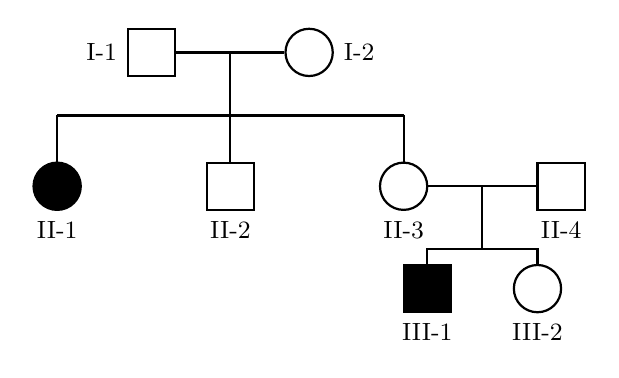
\begin{tikzpicture}[>=Stealth, every node/.style={font=\small}]
  \tikzset{male/.style={draw, thick, minimum size=0.6cm},
           female/.style={draw, thick, circle, minimum size=0.6cm},
           aff/.style={fill=black}}
  % generation I
  \node[male]   (I1) at (1,3.2) {};
  \node[female] (I2) at (3,3.2) {};
  \node[left=0.1] at (I1.west) {I-1};
  \node[right=0.1] at (I2.east) {I-2};
  \draw[thick] (I1) -- (I2);
  \draw[thick] (2,3.2) -- (2,2.4) -- (-0.2,2.4);
  \draw[thick] (2,2.4) -- (4.2,2.4);
  % generation II
  \node[female, aff] (II1) at (-0.2,1.5) {};
  \node[male]        (II2) at (2,1.5) {};
  \node[female]      (II3) at (4.2,1.5) {};
  \node[male]        (II4) at (6.2,1.5) {};
  \foreach \x in {-0.2,2,4.2} {\draw[thick] (\x,2.4) -- (\x,1.8);}
  \draw[thick] (II3) -- (II4);
  \node[below=0.1] at (II1.south) {II-1};
  \node[below=0.1] at (II2.south) {II-2};
  \node[below=0.1] at (II3.south) {II-3};
  \node[below=0.1] at (II4.south) {II-4};
  % generation III
  \draw[thick] (5.2,1.5) -- (5.2,0.7) -- (4.5,0.7) -- (4.5,0.5);
  \draw[thick] (5.2,0.7) -- (5.9,0.7) -- (5.9,0.5);
  \node[male, aff] (III1) at (4.5,0.2) {};
  \node[female]    (III2) at (5.9,0.2) {};
  \node[below=0.1] at (III1.south) {III-1};
  \node[below=0.1] at (III2.south) {III-2};
\end{tikzpicture}
\captionof{figure}{Pedigree of a family with a rare trait.}
\end{center}
\begin{enumerate}
  \item Is the trait dominant or recessive? Justify your answer.
  \item Is the trait autosomal or X-linked? Justify your answer.
  \item Give the genotypes (use $A$ and $a$) of
        \begin{enumerate}
          \item I-1 and I-2,
          \item II-1,
          \item II-3 and II-4.
        \end{enumerate}
  \item What is the probability that III-2 is a carrier of the trait?
\end{enumerate}

% ---- Task 4 ---------------------------------------------------------------------------
\task{4}{Michaelis--Menten kinetics}{8}
The initial rate $v$ of an enzyme-catalysed reaction was measured at different substrate concentrations
$[S]$ (Figure~2). The curve follows the Michaelis--Menten equation
$v = \dfrac{V_{\max}[S]}{K_m + [S]}$.

\begin{center}
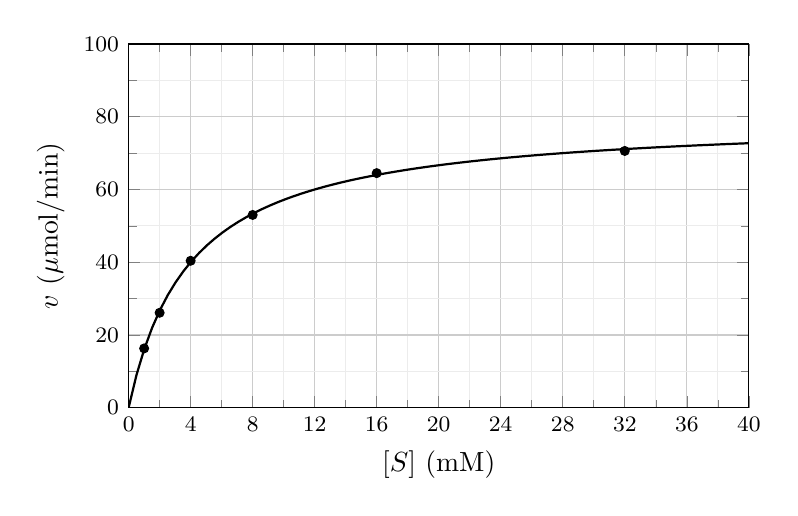
\begin{tikzpicture}
\begin{axis}[width=0.78\linewidth, height=6.2cm,
    xlabel={$[S]$ (mM)}, ylabel={$v$ ($\mu$mol/min)},
    xmin=0, xmax=40, ymin=0, ymax=100,
    xtick distance=4, ytick distance=20, grid=both, minor tick num=1,
    major grid style={gray!40}, minor grid style={gray!15}, tick label style={font=\footnotesize}]
  \addplot[thick, domain=0:40, samples=80] {80*x/(4+x)};
  \addplot[only marks, mark=*, mark size=1.6pt] coordinates
    {(1,16.3) (2,26.1) (4,40.4) (8,53.0) (16,64.5) (32,70.6)};
\end{axis}
\end{tikzpicture}
\captionof{figure}{Initial rate versus substrate concentration.}
\end{center}
\begin{enumerate}[label=(\roman*)]
  \item Estimate $V_{\max}$ and $K_m$ from the graph.
  \item Calculate the initial rate at $[S] = \qty{12}{mM}$ with the Michaelis--Menten equation.
  \item At which substrate concentration does the enzyme reach 90\% of $V_{\max}$?
  \item A competitive inhibitor is added. How do the apparent $K_m$ and $V_{\max}$ change, and why can a high
        substrate concentration overcome the inhibition?
\end{enumerate}

\end{document}
